\part{Discrete Mathematics}
\chapter{Graph Theory}
% Clear this first: https://web.evanchen.cc/notes/SJSU179.pdf
% http://web.mit.edu/yufeiz/www/imo2008/tang-graph.pdf
% https://yufeizhao.com/211/graph_theory_notes.pdf
% https://courses.maths.ox.ac.uk/pluginfile.php/78926/mod_resource/content/0/Lecture%20notes.pdf
% https://books.google.com.cu/books?id=7_bQa4SJTQQC&printsec=frontcover#v=onepage&q&f=false

\section{Definitions}
\subsection{Preliminary Definitions}
\begin{defn}{Graph}{}
A \vocab{graph} $G = (V(G),E(G))$ consists of two sets $V(G)$ (the \textbf{vertex} set) and $E(G)$ (the \textbf{edge} set), where each element of $E(G)$ consists of a pair of elements of $V(G)$. 
\end{defn}

\begin{notation}
$|G|=|V(G)|$ denotes the number of vertices and $e(G) =|E(G)|$ denotes the number of edges.
\end{notation}

The \textbf{order} of a graph $G$ is $|V(G)|$. The \textbf{size} of $G$ is $|E(G)|$.

We represent $G$ visually by drawing a point for each vertex and a line between any pair of points that form an edge.

The \vocab{complement} of $G$, denoted by $\overline{G}$, is a graph with the same vertex set as $G$ and $E(\overline{G}) = \{e \notin E(G)\}$, i.e. $\overline{G}$ has edges exactly where there are no edges in $G$.

\begin{defn}{Simple graph}{}
A loop is an edge $(v,v)$ for some $v \in V$. An edge $e = (u,v)$ is a multiple edge if it appears multiple times in $E$. 

A graph is \vocab{simple} if it has no loops or multiple edges.
\end{defn}

\begin{remark}
Unless explicitly stated otherwise, we will only consider simple graphs. General (potentially non-simple) graphs are also called multigraphs.
\end{remark}

Vertices $u$ and $v$ are \textbf{neighbours} if $(u,v) \in E(G)$; we also say that $u$ and $v$ are \textbf{adjacent}. An edge $e \in E(G)$ is \textbf{incident} to a vertex $v \in V(G)$ if $v \in e$. Edges $e, e^\prime$ are \textbf{incident} if $e \cap e^\prime = \emptyset$.

Given a vertex $v$, the \textbf{degree} of $v$, denoted by $d(v)$, is the number of neighbours of $v$ in $G$. If the degree of each vertex is the same, we can call that the degree of the graph. A \textbf{leaf} is a vertex of degree one, i.e. with a unique neighbour.

\begin{remark}
A trivial graph is a graph with order 1. An empty graph is a graph of size 0. 
Note that a graph must have at least one vertex by definition. But a graph can certainly have no edges!
\end{remark}

\subsection{Subgraph}
\begin{defn}{Subgraph}{}
$H$ is a \vocab{subgraph} of $G$ if $V(H) \subseteq V(G)$ and $E(H) \subseteq E(G)$.
\end{defn}

$H$ is a \vocab{spanning subgraph} if $V(H)=V(G)$.

$H$ is an \vocab{induced subgraph} if $(u,v) \in E(H) \iff (u,v) \in E(G) \forall u, v \in V(H)$.

\subsection{Walks}
\begin{defn}{Walk}{}
A \vocab{$u-v$ walk} in $G$, denoted by $W$, is a finite sequence of vertices $u=v_0,v_1,\dots,v_k=v$ such that $v_i v_{i+1} \in E(G)$ for all $0 \le i < k-1$.
\end{defn}

A walk is \textbf{closed} if and only if $u=v$. Otherwise, it is \textbf{open}.

A \vocab{trail} is an open walk without repeating vertices.

A \vocab{path} is an open walk without repeating edges.
Note that paths are trails, but not vice-versa.

A \vocab{circuit} is a closed walk without repeating edges, i.e. $u=v$, it begins and ends with the same vertex.

A \vocab{cycle} is a closed walk without repeating vertices, other than the initial and terminal vertices, i.e. $u=v$ but the vertices are otherwise distinct and $W$ has at least 3 vertices. If a graph $G$ has no cycle we call it \textbf{acyclic}.

A \vocab{trail} is a walk in which no two vertices appear consecutively (in either order) more than once; that is, no edge is used more than once. A \vocab{tour} is a closed trail.

\subsection{Connectedness}
\begin{defn}{Connected}{}
A graph $G$ is \vocab{connected} if $\forall u,v \in V(G)$ there exists a $u-v$ path.
\end{defn}

Let $G$ be a connected graph. Then $d(u,v)$ is the \textbf{smallest length} of any $u-v$ path if $u \neq v$, or 0 if $u=v$.

The \textbf{diameter} of a connected graph $G$, denoted by $\diam G$, is defined as
\[ \diam G = \max_{u\neq v} d(u,v). \]
By construction, $d(u,v) \le \diam G \forall u,v \in V(G)$.

We say that two vertices $u$ and $v$ of a graph $G$ lie in the same \textbf{component} if they are joined by an $u-v$ walk. Clearly this forms an equivalence relation and the partition of $V(G)$ into equivalence classes expresses $G$ as a union of disjoint connected graphs called its components.

$G$ is \vocab{complete} if every pair of vertices in $G$ is joined by an edge. A complete graph on $n$ vertices is denoted by $K_n$.

\subsection{Classes of graphs}
\vocab{Empty graph}: We let $E_n$ denote the empty graph with order $n$ and size 0. This graph is disconnected if and only if $n \ge 2$.

\vocab{Path graph}: We let $P_n$ be the graph of order $n$ and size $n-1$. You can guess what this is: It is connected with diameter $n-1$.

\vocab{Cycle graph}: We let $C_n$ denote the graph of order $n$ and size $n$ which consists of a single
cycle. Note that $n \ge 3$. It is connected with diameter $\floor{\frac{1}{2}n}$.

\vocab{Complete graph}: We let $K_n$ denote the complete graph, with order $r$ and size $\binom{n}{2}$. It is extremely connected with diameter 1 (for $n \ge 2$). Note that this is the only class of connected graphs with diameter 1.

Note that $E_1 = K_1 = P_1$, $K_2 = P_2$ and $K_3 = C_3$.

\subsection{Bipartite Graphs}
$G$ is \vocab{bipartite} if $V(G)$ can be partitioned into two non-empty disjoint sets $A$ and $B$ such that no edge has both endpoints in the same set. A graph is said to be \textbf{complete bipartite} if $G$ is bipartite and all possible edges between the two sets $A$ and $B$ are drawn. In the case where $|A|=m, |B|=n$, such a graph is denoted by $K_{m,n}$.

Let $k \ge 2$. A graph $G$ is said to be \textbf{$k$-partite} if $V(G)$ can be partitioned into $k$ pairwise disjoint sets $A_1, \dots, A_k$ such that no edge has both endpoints in the same set. A \textbf{complete $k$-partite} graph is defined similarly as a complete bipartite. In the case where $|A_i| = n_i$, such a graph is denoted by $K_{n_1,n_2,\dots,n_k}$.

A graph is \vocab{planar} if it can be drawn such that a pair of edges can only cross at a vertex.

\begin{thrm}{Euler's Characteristic Formula}{}
For any connected planar graph, the number of vertices $V$ minus the number of edges $E$ plus the number of regions $R$ equals 2. 
\begin{equation} V-E+R = 2 \end{equation}
\end{thrm}

(or V-E+F=2 for 3 dimensional polyhedra)
To prove this, 
for trivial graph, V=1, F=1, E=0
Adding one edge, we either introduce a new vertex or face (if edge is connected to preexisting vertex)



\subsection{Isomorphism}
\begin{defn}{Isomorphism}{}
Let $G_1 = (V_1, E_1)$ and $G_2 = (V_2, E_2)$ be graphs. An isomorphism $\phi : G_1 \to G_2$ is a bijection (a one-to-one correspondence) from $V_1$ to $V_2$ such that $(u,v) \in E_1$ if and only if $(\phi(u),\phi(v)) \in E_2$. We say $G_1$ is isomorphic to $G_2$ if there is an isomorphism between them.
\end{defn}



\section{Trees and Balancing}
A \vocab{tree} is defined to be a connected graph that does not contain any cycles; to put it simply, it is a minimally connected graph.

A \vocab{cycle} in a graph means there is a path from an object back to itself.

Characterisation of trees: Let $G$ be a connected graph with $n$ vertices. The following statements are equivalent.
\begin{enumerate}
\item $G$ does not contain any cycles
\item $G$ contains exactly $n-1$ edges
\item For any two vertices, there exists exactly one path joining the two vertices
\item The removal of any edge disconnects the graph
\end{enumerate}

\begin{lemma}\label{acyclic}
Any tree is acyclic.
\end{lemma}
\begin{proof}
Let $G$ be a tree, i.e. $G$ is minimally connected. Suppose for a contradiction that $G$ contains a cycle $C$. Let $e \in E(C)$. We will obtain our contradiction by showing that $G-e \coloneqq (V(G),E(G)\setminus\{e\})$ is connected. 

Let $P$ be the path obtained by deleting $e$ from $C$. Consider any $u,v$ in $V(G)$. As $G$ is connected, there is an $u-v$ walk $W$ in $G$. Replacing any use of $e$ in $W$ by $P$ gives an $u-v$ walk in $G-e$. Thus $G-e$ is connected, a contradiction.
\end{proof}

There are many equivalent characterisations of trees, any of which could be taken as the definition. Here is one:

\begin{lemma}\label{tree_iff}
$G$ is a tree if and only if $G$ is connected and acyclic.
\end{lemma}
\begin{proof}
If $G$ is a tree then $G$ is connected by definition and acyclic by \cref{acyclic}. Conversely, let $G$ be connected and acyclic. Suppose for a contradiction that $G-e$ is connected for some $e = (u,v) \in E(G)$.

Let $W$ be a shortest $u-v$ walk in $G-e$. Then $W$ must be a path, i.e. have no repeated vertices, otherwise we would find a shorter walk by deleting a segment of $W$ between two visits to the same vertex. Combining $W$ with $(u,v)$ gives a cycle, which is a contradiction.
\end{proof}

\begin{remark}
The fact that a shortest walk between two points is a path is often useful. More generally, considering an extremal (shortest, longest, minimal, maximal, \dots) object is often a useful proof technique.
\end{remark}

\begin{lemma}
Any two vertices in a tree are joined by a unique path.
\end{lemma}
\begin{proof}
Suppose for a contradiction that this fails for some tree $G$. 

Choose $u,v$ in $V(G)$ so that there are distinct $u-v$ paths P1, P2, and P1 is as short as possible over all such choices of $u$ and $v$.

Then P1 and P2 only intersect in $u$ and $v$, so their union is a cycle, contradicting \cref{acyclic}.
\end{proof}

\begin{lemma}\label{tree_leaves}
Any tree with at least two vertices has at least two leaves.
\end{lemma}
\begin{proof}
Consider any tree $G$. Let $P$ be a longest path in $G$. The two ends of $P$ must be leaves. Indeed, an end cannot have a neighbour in $V(G) \setminus V(P)$, or we could make $P$ longer, and cannot have any neighbour in $V(P)$ other than the next in the sequence of $P$, or we would have a cycle.

The existence of leaves in trees is useful for inductive arguments, via the following lemma. Given $v \in V(G)$, let $G-v$ be the graph with $V(G-v) = V(G)\setminus\{v\}$ and $E(G-v) = \{(u,v) \in E(G) \mid v \notin \{u,v\}\}$.
\end{proof}

\begin{lemma}\label{tree_leaf}
If $G$ is a tree and $v$ is a leaf of $G$ then $G-v$ is a tree.
\end{lemma}
\begin{proof}
By \cref{tree_iff} it suffices to show that $G-v$ is connected and acyclic. Acyclicity is immediate from \cref{acyclic}. Connectedness follows by noting for any $u,v \in V(G)\setminus\{v\}$ that the unique $u-v$ path in $G$ is contained in $G-v$.
\end{proof}

\begin{lemma}\label{tree_edges}
Any tree on $n$ vertices has $n-1$ edges.
\end{lemma}
\begin{proof}
By induction. A tree with 1 vertex has 0 edges. Let $G$ be a tree on $n>1$ vertices. By \cref{tree_leaves}, $G$ has a leaf $v$. By \cref{tree_leaf}, $G-v$ is a tree. By induction hypothesis, $G-v$ has $n-2$ edges. Replacing $v$ gives $n-1$ edges in $G$.
\end{proof}

We conclude this section with another characterisation of trees. First we note that any connected graph $G$ contains a minimally connected subgraph (i.e. a tree) with the same vertex set, which we call a \vocab{spanning tree} of $G$.

\begin{lemma}
A graph $G$ is a tree on $n$ vertices if and only if $G$ is connected and has $n-1$ edges.
\end{lemma}
\begin{proof}
If $G$ is a tree then $G$ is connected by definition and has $n-1$ edges by \cref{tree_edges}. 

Conversely, suppose that $G$ is connected and has $n-1$ edges. Let $H$ be a spanning tree of $G$. Then $H$ has $n-1$ edges by \cref{tree_edges}, so $H = G$, so $G$ is a tree.
\end{proof}

\section{Euler Tours and Trails}
An \vocab{Euler trail} is a trail in which every pair of adjacent vertices appear consecutively. (That is, every edge is used exactly once.)

An \vocab{Euler tour} is a closed Euler trail.


vertex/edge colouring and Ramsey Theory

Regular graph
Directed graph

graph concepts such as Shortest-, Euler-, Hamilton-Paths and Cycles, coloring, planarity, weighted graphs, and directed graphs.

Topics in graph theory, including: connectivity and matchings, Hall's theorem, Menger's theorem, network flows; paths and cycles, complete subgraphs and Turán's theorem, and the Erdös-Stone theorem; graph colouring and the four-colour theorem; Ramsey theory; probabilistic methods in graph theory; and the use of software to solve graph-theoretic problems.
\pagebreak

\section*{Problems}
\begin{prbm}[K\"{o}nigsberg Bridge Problem]
K\"{o}nigsberg was a small town in Prussia. There is a river running through the town and there were seven bridges across the river. The inhabitants of K\"{o}nigsberg liked to walk around the town and cross all of the bridges:

Is it possible to walk around the town and cross every bridge, once and once only?
\end{prbm}

\begin{solution}
We replace every landmass by a vertex and every bridge by an edge to give the following graph.


\end{solution}
\pagebreak

Problems can include tournament, matching, and scheduling problems.
\begin{prbm}(Moser's circle problem) 
Determine the number of regions into which a circle is divided if $n$ points on its circumference are joined by chords with no three internally concurrent.
\end{prbm}

\begin{proof}[Solution]
Consider the graph which has points on the circumference and intersection points between chords as its vertices.

Let $V, E, F$ denote the number of vertices, edges, regions respectively.

To count the number of intersection points, note that $4$ points on the circumference give one unique intersection point between the two non-parallel chords formed by connecting two pairs of points which intersect inside the circle. Hence, number of intersection points is $\dbinom{n}{4}$. 
\[ V = n + \binom{n}{4} \]
Total number of edges includes $n$ circular arcs, number of original chords formed from connecting pairs of points on the circumference
E = no. of original lines + 2 x no. of intersection points
E = n choose 2 + 2 x n choose 4 + n
since there are n circular arcs

Using Euler's Characteristic Formula, we have 
\begin{align*}
F &= E - V - 1 \\
\Aboxed{F &= 1 + \binom{n}{2} + \binom{n}{4}}
\end{align*}
\end{proof}

\chapter{Game Theory}
\textbf{Recommended readings:} \href{https://mathematicalolympiads.files.wordpress.com/2012/08/martin_j-_osborne-an_introduction_to_game_theory-oxford_university_press_usa2003.pdf}{``An Introduction to Game Theory" by Osborne}

% games of normal form and extensive form, and their applications in economics, relations between game theory and decision making; games of complete information: static games with finite or infinite strategy spaces, Nash equilibrium of pure and mixed strategy, dynamic games, backward induction solutions, information sets, subgame-perfect equilibrium, finitely and infinitely-repeated games; games of incomplete information: Bayesian equilibrium, first price sealed auction, second price sealed auction, and other auctions, dynamic Bayesian games, perfect Bayesian equilibrium, signaling games; cooperative games: bargaining theory, cores of n-person cooperative games, the Shapley value and its applications in voting, cost sharing, etc.

Game Theory is the study of strategically interdependent behaviour.
\section{Strict Dominance}
\subsection{Prisoner's Dilemma}
To start off, we will take a look at the \vocab{Prisoner's Dilemma}, which goes as follows:

\begin{ebox}
Two thieves plan to rob a store, but the police arrest them for trespassing. The police suspect that they planned to break in but lack the evidence to support such an accusation. They require a confession to charge the suspects. The police offer them the following deal:
\begin{itemize}
\item If no one confesses, both are charged a \emph{one month} jail sentence each for trespassing.
\item If a rat confesses and the other does not, the rat is not charged but the other is charged a \emph{twelve month} jail sentence for robbery.
\item If both confess, both are charged an \emph{eight month} jail sentence each.
\end{itemize}
If both criminals are self-interested and only care about minimising their jail time, should they take the interrogator's deal?
\end{ebox}

We condense the above information into a \vocab{payoff matrix} as shown below, where we have two players, A and B. The horizontal rows represent A's choices, while the vertical columns represent B's choices, and each cell contains a combination of their payoffs.

\begin{table}[H]
\centering
\begin{tabular}{rcc}
\multicolumn{1}{l}{}         & quiet                       & confess                     \\ \cline{2-3} 
\multicolumn{1}{r|}{quiet}   & \multicolumn{1}{c|}{$-1$, $-1$} & \multicolumn{1}{c|}{$-12$, $0$} \\ \cline{2-3} 
\multicolumn{1}{r|}{confess} & \multicolumn{1}{c|}{$0$, $-12$} & \multicolumn{1}{c|}{$-8$, $-8$} \\ \cline{2-3} 
\end{tabular}
\end{table}

\subsection{Split or Steal}
The game goes as follows:
\begin{ebox}
Each of two players, Sarah and Steve, has to pick one of two balls: inside one ball appears the word ‘\textbf{split}’ and inside the other the word ‘\textbf{steal}’ (each player is first asked to secretly check which of the two balls in front of him/her is the split ball and which is the steal ball). They make their decisions simultaneously. 
\end{ebox}

The possible outcomes are shown in the figure below, where each row is labelled with a possible choice for Sarah and each column with a possible choice for Steven. Each cell in the table thus corresponds to a possible pair of choices and the resulting outcome is written inside the cell.

\begin{figure}[H]
    \centering
    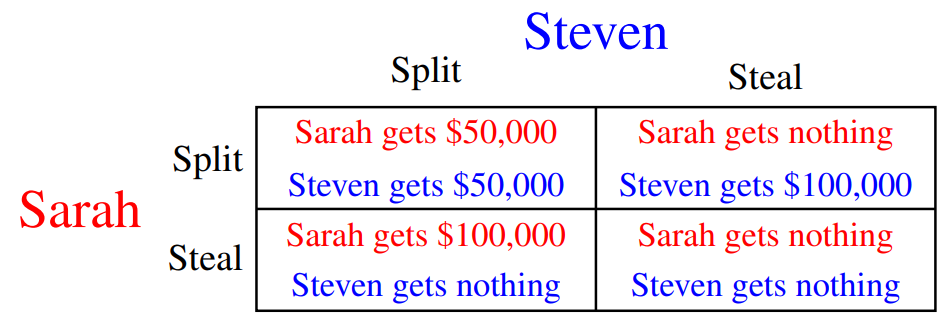
\includegraphics[width=12cm]{images/Split_or_steal.png}
\end{figure}

\section{Nash Equilibrium}
\textbf{Nash Equilibrium} is a set of optimal strategies that work against \textit{all} counter-steategies. This means that if any given player were told the strategies of all their opponents, they still would choose to retain their original strategy. 

\subsection{Matrix games}

\section{Fair Division}
\subsection{Rental harmony problem}
Sperner's lemma

https://www.cs.cmu.edu/~arielpro/15896/docs/paper19b.pdf
